\hyperdef{}{tilda}{}

\subsection{\texorpdfstring{{Sprachwandel}}{Sprachwandel}}

\subsubsection{\texorpdfstring{{Sprachen}}{Sprachen}}

\vspace{0.5cm}\par\noindent\textbf{Der Nordwind und die Sonne und das Problem der Sprachgrenzen}\vspace{0.5cm}

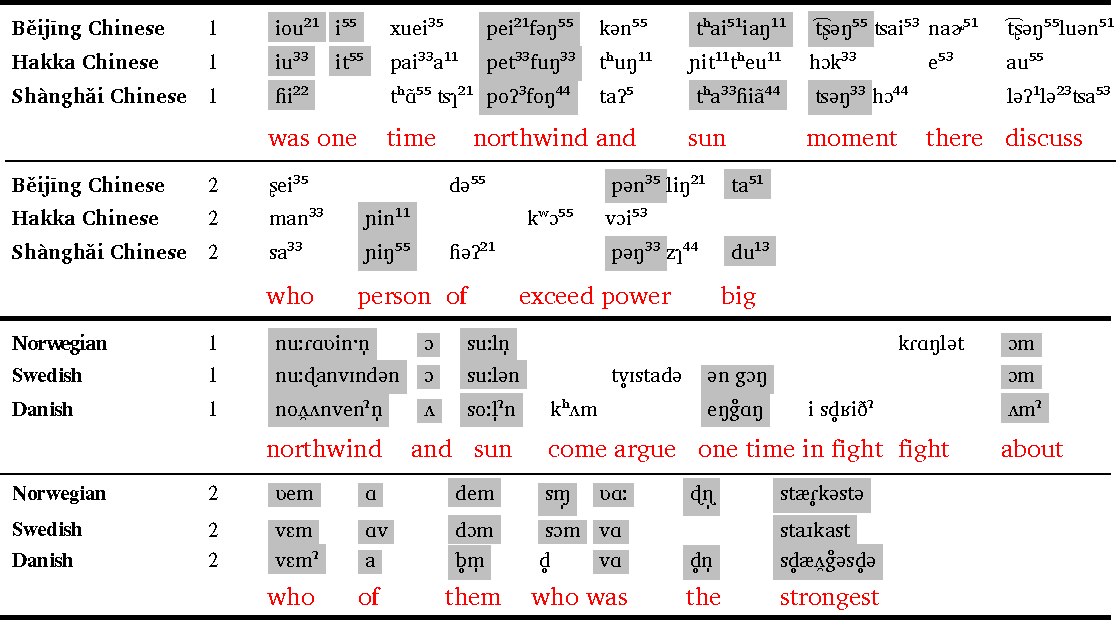
\includegraphics[width=\textwidth]{img/northwind.pdf}

\vspace{0.5cm}\par\noindent\textbf{Diasysteme}\vspace{0.5cm}

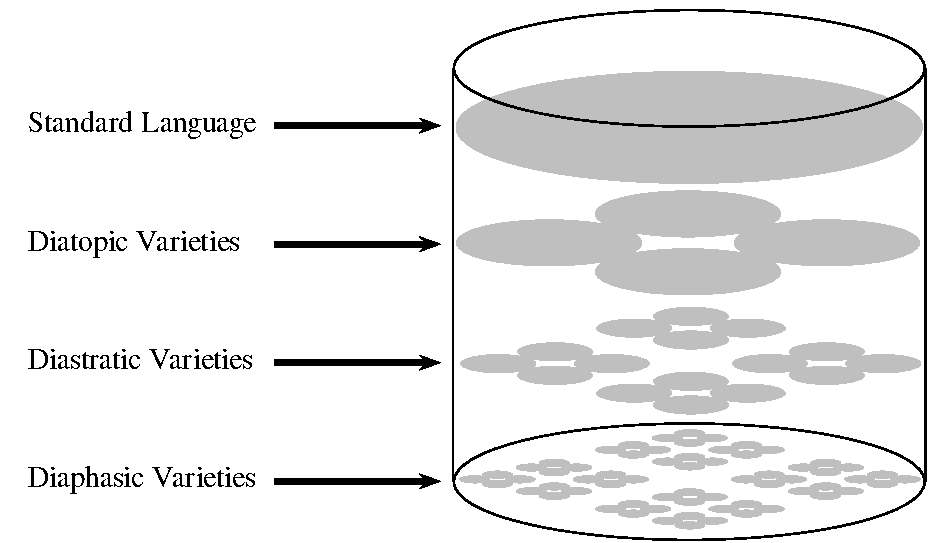
\includegraphics[width=\textwidth]{img/diasystem.pdf}

\vspace{0.5cm}\par\noindent\textbf{Dimensionen der Sprachvariation}\vspace{0.5cm}

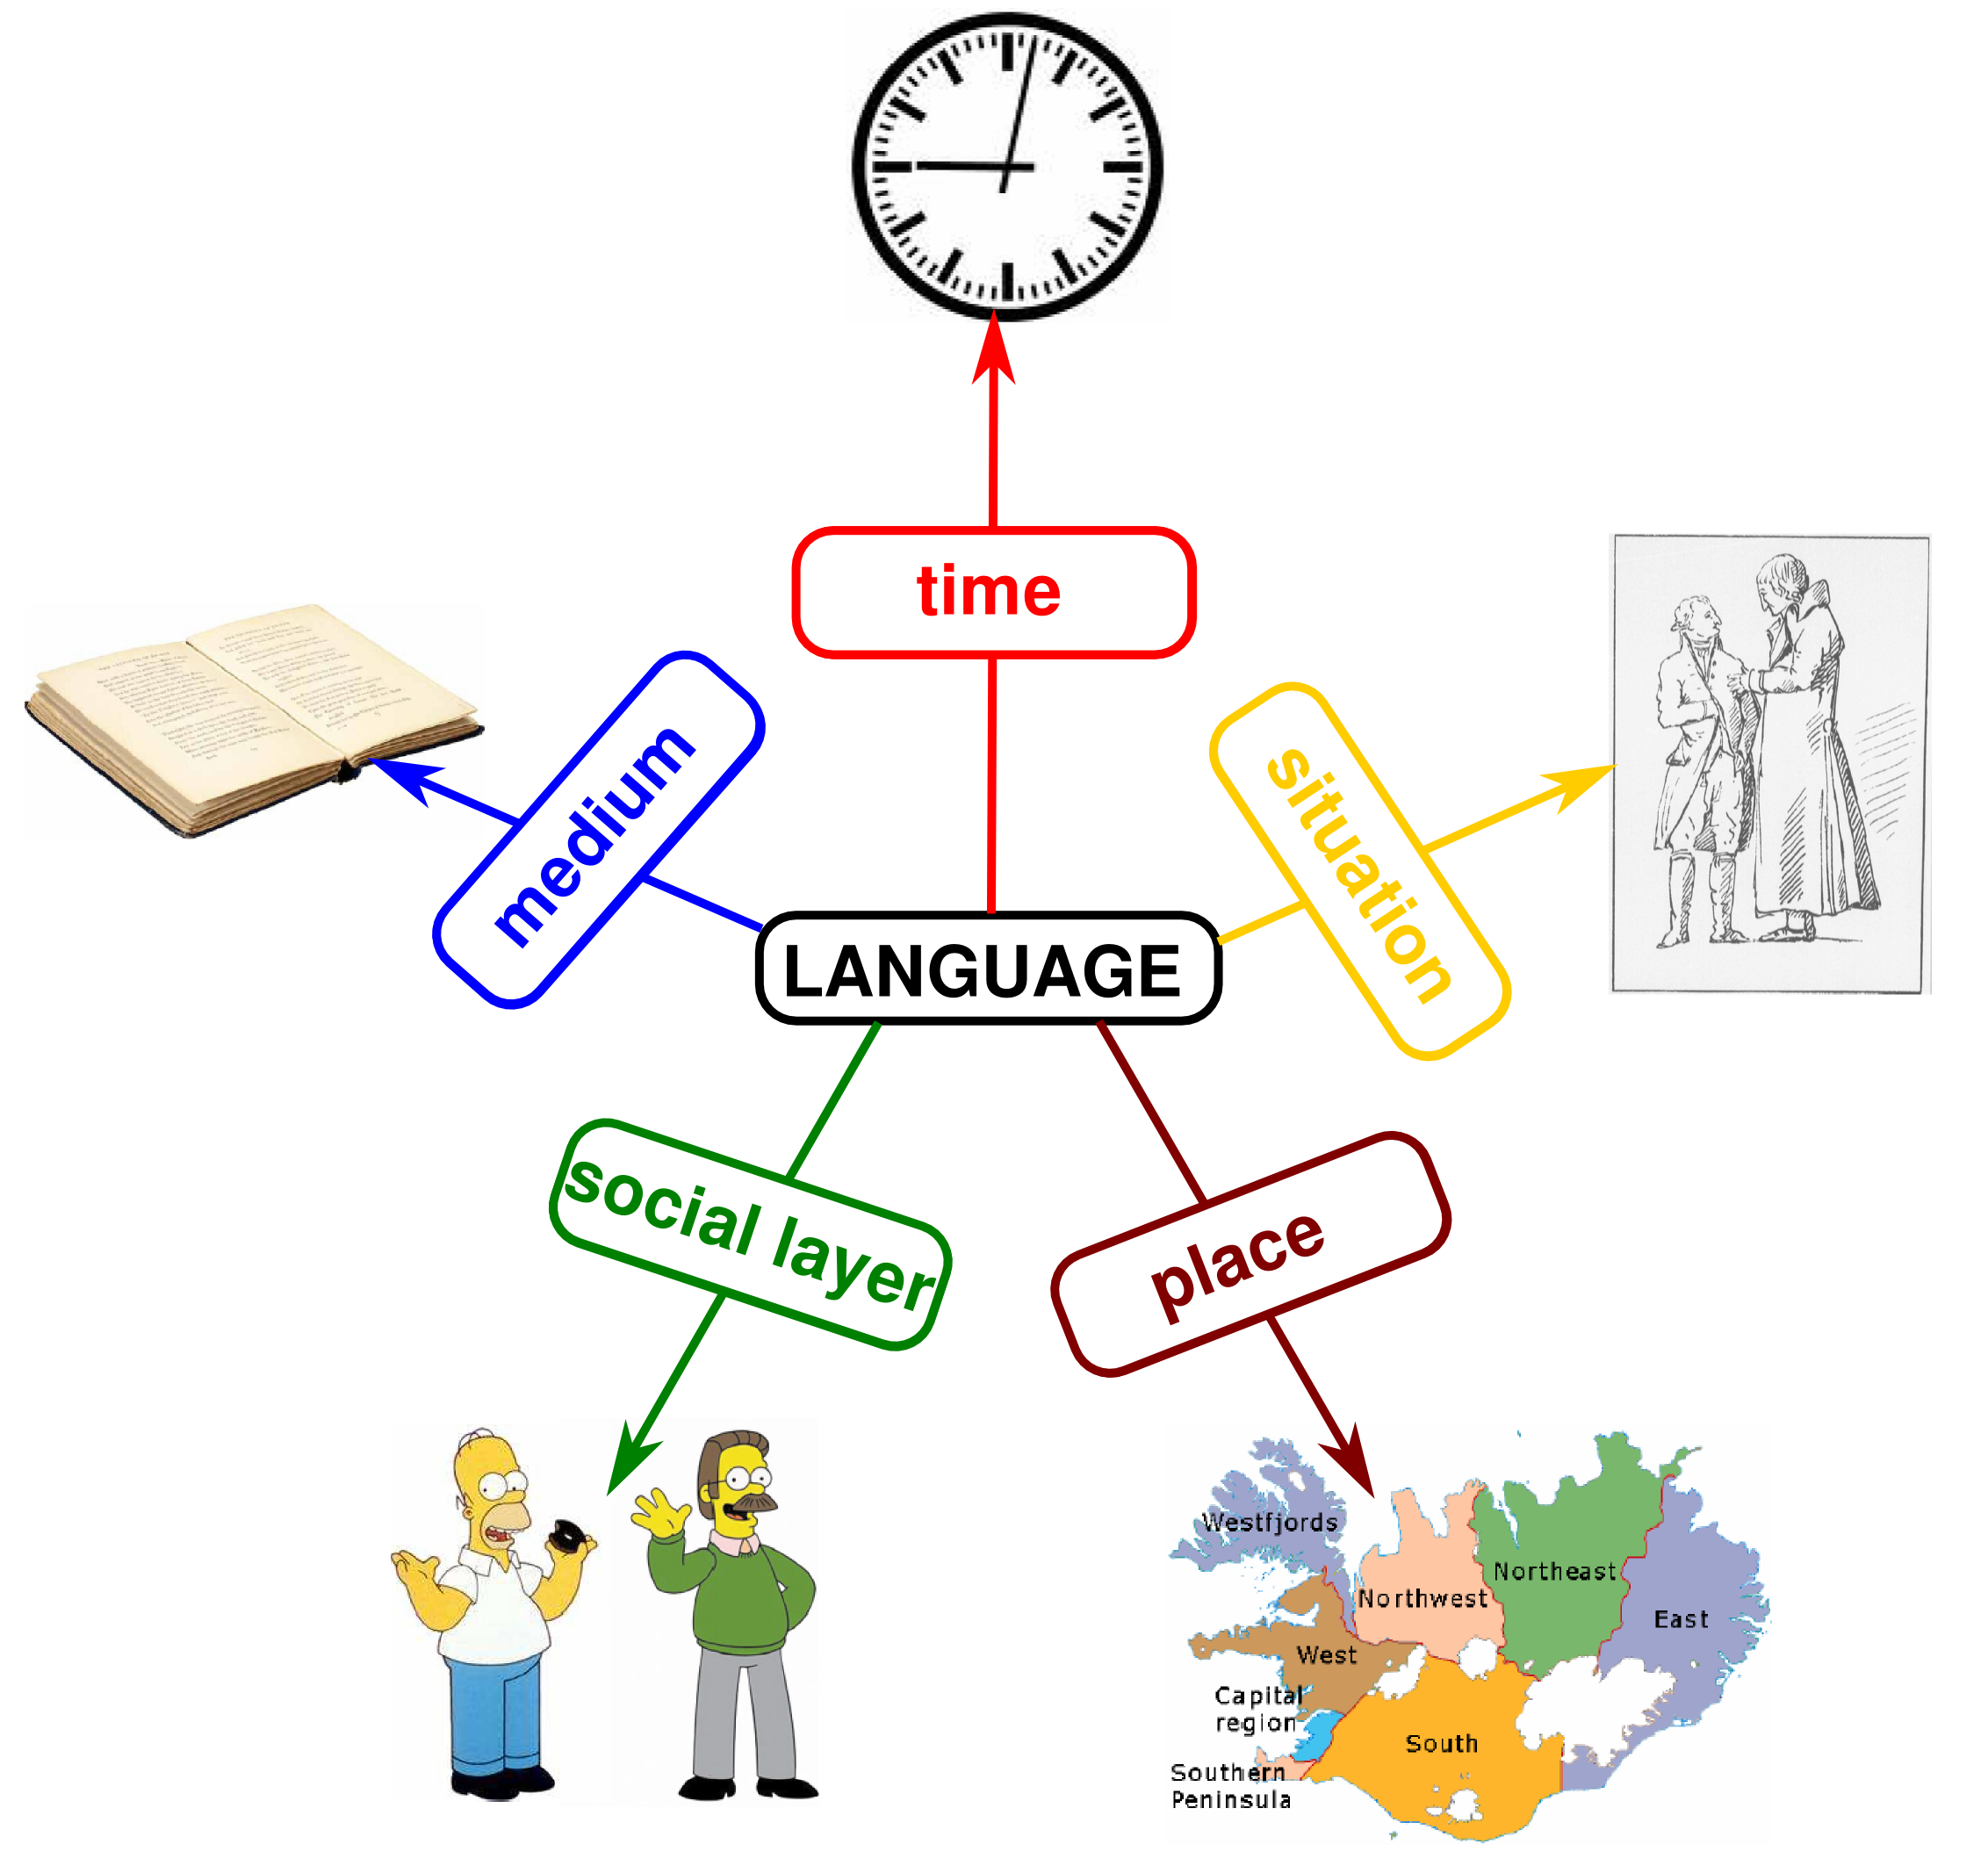
\includegraphics[width=\textwidth]{img/variation-1.png}

\vspace{0.5cm}\par\noindent\textbf{Komplexität des Sprachwandels}\vspace{0.5cm}

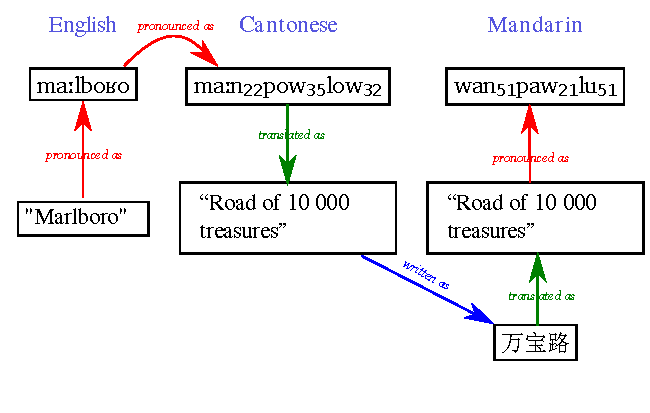
\includegraphics[width=\textwidth]{img/marlboro.pdf}

\subsubsection{\texorpdfstring{{Sprachwandel im
Allgemeinen}}{Sprachwandel im Allgemeinen}}

\vspace{0.5cm}\par\noindent\textbf{Die komischen Reime in den chinesischen Oden}\vspace{0.5cm}

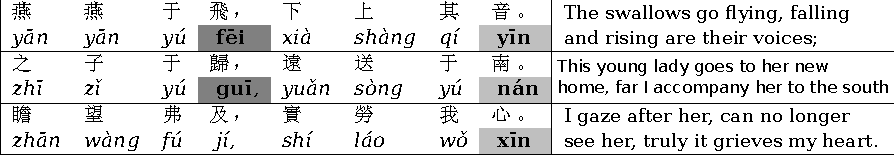
\includegraphics[width=\textwidth]{img/odes.pdf}


\vspace{0.5cm}\par\noindent\textbf{Die komischen Reime in den chinesischen Oden}\vspace{0.5cm}

\begin{quote}
The writings of scholars must be made of adequate sounds. Even in the
rural areas everybody orders the sounds harmonically. Can it be that the
ancients solely did not have rhymes? One can say that in the same way in
which ancient times differ from modern times, and places in the North
differ from places in the South, characters change and sounds shift.
This is a natural tendency. Therefore, it is inevitable that reading the
ancient writings with modern pronun- ciation will sound improper and
wrong. (Máoshī Gǔyīnkǎo: 原序, meine Übersetzung)
\end{quote}

\vspace{0.5cm}\par\noindent\textbf{Wandel als Katastrophe}\vspace{0.5cm}

Schon früh in der Geschichte der Linguistik war den Forschern in Europa
bewusst, dass Sprachen sich wandeln können. Vorherrschend war dabei
jedoch die Ansicht, dass alle Formen des Wandels ``katastrophisch''
abliefen, dass Wandel also im Rahmen eines unberechenbaren, chaotischen
``Verfalls'' vor sich ginge. Erst spät (zu Beginn des 19. Jahrhunderts)
wurde erstmals klar, dass sich bestimmte Phänomene des Sprachwandels,
insbesondere der Lautwandel, durch eine beachtliche Regelmäßigkeit
auszeichnen.

\vspace{0.5cm}\par\noindent\textbf{Wandel als Prozess}\vspace{0.5cm}

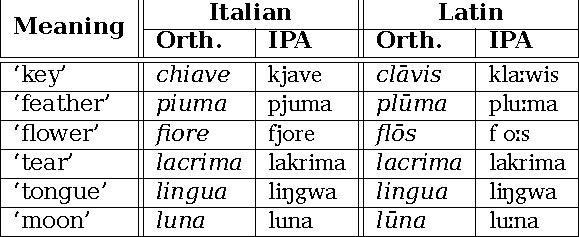
\includegraphics[width=\textwidth]{img/lautwandel-ita-lat.pdf}



\vspace{0.5cm}\par\noindent\textbf{Wandel und Regelmäßigkeit}\vspace{0.5cm}

Während den Menschen im Verlaufe der Geschichte bereits relativ lange
bewusst war, dass Sprachen sich ändern können, war es eine radikal neue
Erkenntnis, die sich zu Beginn des 19. Jahrhunderts
herauskristallisierte, dass Sprachen sich in Prozessen ändern, von denen
bestimmte sogar regelmäßig verlaufen können. Mit der Entdeckung der
Regelmäßigkeit einher festigte sich ebenfalls die Erkenntnis, dass
Sprachen miteinander verwandt sein können, wobei Verwandtschaft von
Sprachen dadurch definiert ist, dass miteinander verwandte Sprachen aus
einer gemeinsamen Vorgängersprache entstanden sind, wie bspw. das
Englische und das Deutsche, die beide aus dem Protogermanischen
hervorgegangen sind.


\subsubsection{\texorpdfstring{{Lautwandel}}{Lautwandel}}

\vspace{0.5cm}\par\noindent\textbf{Wandel als Gesetz\vspace{0.5cm}
(\href{http://bibliography.lingpy.org?key=Osthoff1878}{Osthoff und
Brugmann 1878: XIII})}

\begin{quote}
Aller lautwandel, soweit er mechanisch vor sich geht, vollzieht sich
nach ausnahmslosen gesetzen, d.h. die richtung der lautbewegung ist bei
allen angehörigen einer sprachgenossenschaft, ausser dem Fall, dass
dialektspaltung eintritt, stets dieselbe, und alle wörter, in denen der
der lautbewegung unterworfene laut unter gleichen verhältnissen
erscheint, werden ohne ausnahme von der änderung ergriffen.
\end{quote}



\vspace{0.5cm}\par\noindent\textbf{Chaque mot a son histoire}\vspace{0.5cm}

Nicht alle Linguisten waren der Meinung der Junggrammatiker. Besonders
Dialektologen folgten dem berühmten Slogan \emph{chaque mot a son
histoire} (``jedes Wort hat seine Geschichte''), der gewöhnlich
\href{http://de.wikipedia.org/wiki/Jules_Gilliéron}{Jules Gilliéron
(1854--1926)} zugeschrieben wird
(\href{http://bibliography.lingpy.org?key=Campbell1999}{Campbell 1999:
189}). Die Bedenken der Dialektologen standen jedoch strengenommen nicht
direkt im Widerspruch zur junggrammatischen Doktrin, schließlich besagte
die junggrammatische Theorie ja nicht, dass sich zwangsläufig
\emph{alle} Wörter einer Sprache regelmäßig änderten, sondern lediglich,
dass idiosynkratischer Wandel durch andere Mechanismen (Entlehnung oder
Analogie) erklärt werden konnte
(\href{http://bibliography.lingpy.org?key=Kiparsky1988}{Kiparsky
1988:368}).

\subsection{\texorpdfstring{{Lautwandel}}{Lautwandel}}

\subsubsection{\texorpdfstring{{Mechanismen des
Lautwandels}}{Mechanismen des Lautwandels}}

\vspace{0.5cm}\par\noindent\textbf{Junggrammatischer Lautwandel (nach\vspace{0.5cm}
\href{http://bibliography.lingpy.org?key=Wang2006a}{Wang 2006: 109,
meine Übersetzung})}

\begin{quote}
Regarding the lexicon {[}they assumed{]} that a change always affects
the whole lexicon, and can therefore be seen as an abrupt change.
Regarding the sounds {[}they assumed{]} that the change proceeded step
by step, and can therefore be seen as a gradual change.
\end{quote}


\vspace{0.5cm}\par\noindent\textbf{Lexikalische Diffusion\vspace{0.5cm}
(\href{http://bibliography.lingpy.org?key=Wang1969}{Wang 1969: 9})}

\begin{quote}
Phonological change may be implemented in a manner that is phonetically
abrupt but lexically gradual. As the change diffuses across the lexicon,
it may not reach all the morphemes to which it is applicable. If there
is another change competing for part of the lexicon, residue may result.
\end{quote}

\vspace{0.5cm}\par\noindent\textbf{Kompettitierende Theorien der Lautwandelmechanismen}\vspace{0.5cm}

\tabular{lll}
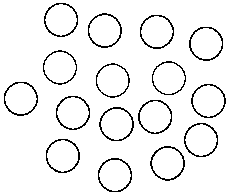
\includegraphics[width=0.25\textwidth]{img/neo-0.png} &
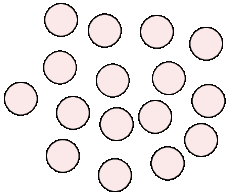
\includegraphics[width=0.25\textwidth]{img/neo-1.png} &
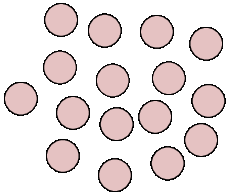
\includegraphics[width=0.25\textwidth]{img/neo-2.png} \\
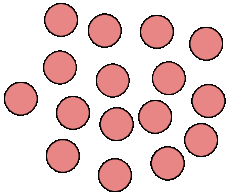
\includegraphics[width=0.25\textwidth]{img/neo-3.png} &
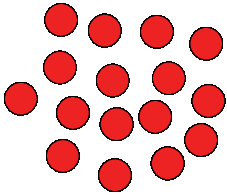
\includegraphics[width=0.25\textwidth]{img/neo-4.png} &
\\
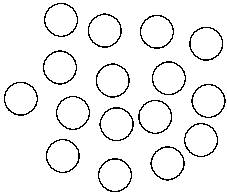
\includegraphics[width=0.25\textwidth]{img/diffusion-0.png} &
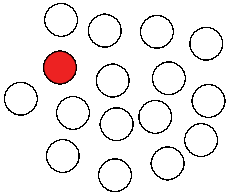
\includegraphics[width=0.25\textwidth]{img/diffusion-1.png}&
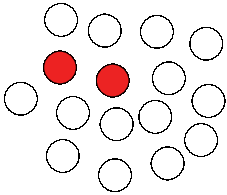
\includegraphics[width=0.25\textwidth]{img/diffusion-2.png}\\
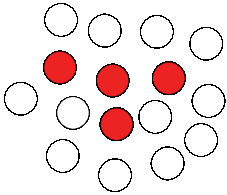
\includegraphics[width=0.25\textwidth]{img/diffusion-3.png}&
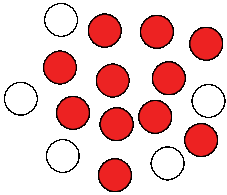
\includegraphics[width=0.25\textwidth]{img/diffusion-4.png}&
\\
\endtabular



\vspace{0.5cm}\par\noindent\textbf{Zwei Mechanismen des Lautwandels\vspace{0.5cm}
(\href{http://bibliography.lingpy.org?key=Labov1994}{Labov 1994: 471})}

\begin{quote}
There is no basis for contending that lexical diffusion is somehow more
fundamental than regular, phonetically motivated sound change. On the
contrary, if we were to decide the issue by counting cases, there appear
to be far more substantially documented cases of Neogrammarian sound
change than of lexical diffusion.
\end{quote}


\subsubsection{\texorpdfstring{{Typen des
Lautwandels}}{Typen des Lautwandels}}

\vspace{0.5cm}\par\noindent\textbf{Terminologische Probleme}\vspace{0.5cm}

Die lange Forschungstradition in der historischen Linguistik hat zur
Postulierung einer Vielzahl unterschiedlicher Typen des Lautwandels\}
geführt. Leider ist die Terminologie, welche verwendet wird, um auf
diese Typen in der Literatur zu verweisen, etwas ``unstetig'' und reicht
von sehr konkreten Termini, welche sehr konkrete Lautwandelinstanzen
abdecken, bis hin zu sehr generellen Termini, die auf den Wandel
abstrakter Lautklassen verweisen.



\vspace{0.5cm}\par\noindent\textbf{Terminologische Probleme}\vspace{0.5cm}

Was in der Literatur als \emph{Lautwandeltyp} bezeichnet wird, kann
dabei sowohl das Phänomen des \emph{Rhotazismus} umfassen
(\href{Trask2000}{Trask 2000: 288}), welches, vereinfacht gesagt, einen
Wandel von /s/ nach /r/ bezeichnet, als auch den Prozess der
\emph{Lenisierung}, welcher eine bestimmte Art von Wandel bezeichnet,
``in which a segment becomes less consonant-like than previously''
(\href{Trask2000}{idb. 190}).



\vspace{0.5cm}\par\noindent\textbf{Definitionen von\vspace{0.5cm}
\href{http://bibliography.lingpy.org?key=Trask2000}{Trask (2000}}

\begin{itemize}
\itemsep1pt\parskip0pt\parsep0pt
\item
  \textbf{Assimilierung} "Any \textbf{syntagmatic change} in which some
  segment becomes more similar in nature to antother segment int he same
  sequence, usually within a single phonological word or phrase" (30).
\item
  \textbf{Dissimilierung} "Any \textbf{syntagmatic change} in which one
  segment changes so as to become less similar to another segment in the
  same form" (95).
\item
  \textbf{Metathese} "Any \textbf{syntagmatic change} in which the order
  of segments (or simetimes of other phonological elements) in a word is
  altered" (211).
\item
  \textbf{Tonogenese} ``Any process which leads to the introduction of
  tones into a language which formerly lacked them'' (346).
\end{itemize}



\vspace{0.5cm}\par\noindent\textbf{Definitionen von\vspace{0.5cm}
\href{http://bibliography.lingpy.org?key=Trask2000}{Trask (2000,
cont.)}}

\begin{itemize}
\itemsep1pt\parskip0pt\parsep0pt
\item
  \textbf{Sandhi} "Any of various phonological processes applying to
  sequences of segments either across morpheme boundaries
  (\emph{internal sandhi}) or across word boundaries (\emph{external
  sandhi})" (296).
\item
  \textbf{Haplologie} ``A type of phonological change (of or
  phonological constraint) in which one of two adjacent syllables of
  identical or similar form is lost (or fails to appear in the first
  place)'' (146).
\item
  \textbf{Elision (Aphaerese, Synkope, Apokope)} "Any of various
  processes in which phonological segments are lost from a word or a
  phrase. Specific varieties of elision are often given special names
  like \textbf{aphaeresis}, \textbf{syncope}, \textbf{apocope,
  synaeresis, synizesis, synaloepha}. Not infrequently this name is
  given to specific processes in particular languages" (102).
\end{itemize}



\vspace{0.5cm}\par\noindent\textbf{Definitionen von\vspace{0.5cm}
\href{http://bibliography.lingpy.org?key=Trask2000}{Trask (2000,
cont.)}}

\begin{itemize}
\itemsep1pt\parskip0pt\parsep0pt
\item
  \textbf{Epenthese} ``Any phonological change which inserts a segment
  into a word or form in a position in which no segment was formerly
  present'' (107).
\item
  \textbf{Prothese} "The addition of a segment to the beginning of a
  word. {[}\ldots{}{]} The opposite is \textbf{aphaeresis}" (266).
\item
  \textbf{Nasalierung} ``Any phonological process in which a segment
  acquires a nasal character which it formerly lacked'' (224).
\end{itemize}

\subsubsection{\texorpdfstring{{Typen des
Lautwandels}}{Typen des Lautwandels}}

\vspace{0.5cm}\par\noindent\textbf{Ein vereinfachtes Modell}\vspace{0.5cm}

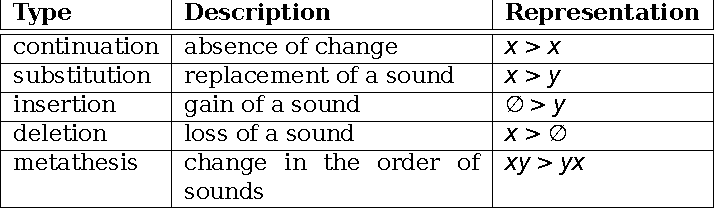
\includegraphics[width=\textwidth]{img/indel.pdf}

\subsection{\texorpdfstring{{Lautwandel}}{Lautwandel}}

\subsubsection{\texorpdfstring{{Typen des
Lautwandels}}{Typen des Lautwandels}}

\vspace{0.5cm}\par\noindent\textbf{Ein vereinfachtes Modell (Beispiele)}\vspace{0.5cm}

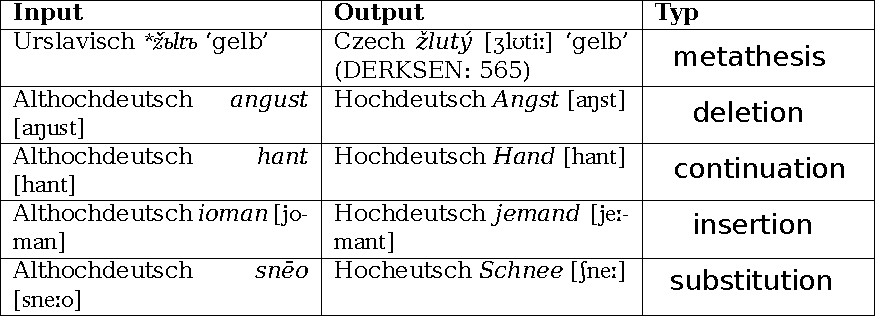
\includegraphics[width=\textwidth]{img/indel-concrete.pdf}


\subsubsection{\texorpdfstring{{Die komparative
Methode}}{Die komparative Methode}}

\vspace{0.5cm}\par\noindent\textbf{Definitionen}\vspace{0.5cm}

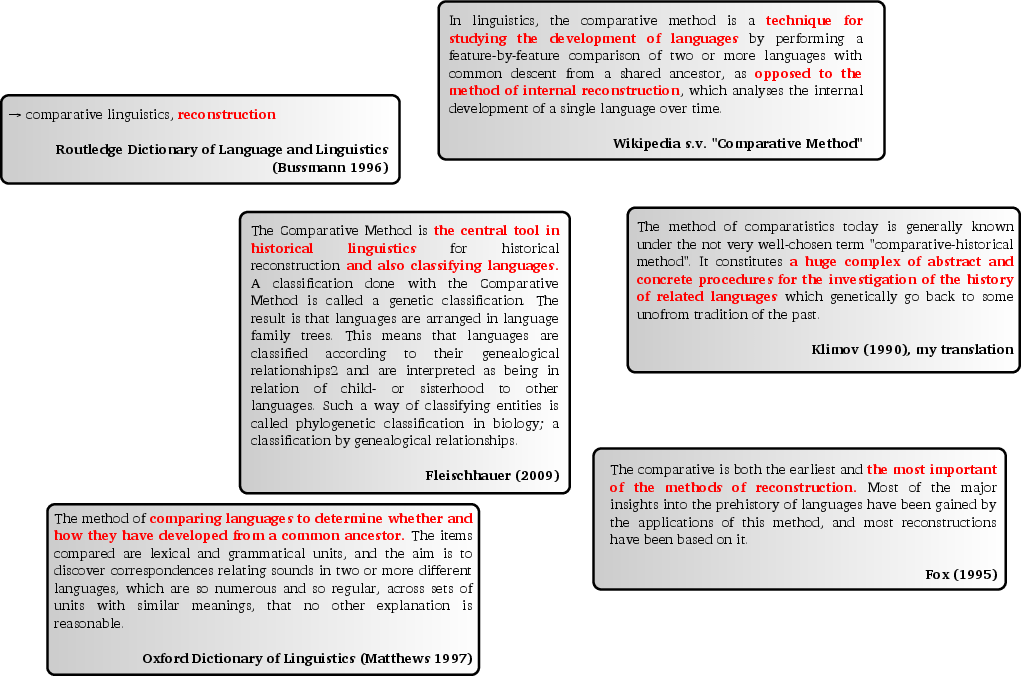
\includegraphics[width=\textwidth]{img/cm-wirr.png}



\vspace{0.5cm}\par\noindent\textbf{Ein neuer Definitionsversuch}\vspace{0.5cm}

Die komparative Methode ist ein Komplex von Verfahren der historischen
Sprachwissenschaft, mit deren Hilfe Sprachen klassifiziert und nicht
belegte Sprachstufen rekonstruiert werden, um somit
Entwicklungsgeschichte von Sprachen zu schreiben. Die Ergebnisse der
komparativen Methoden werden in Form von etymologischen Wörterbüchern,
historischen Grammatiken und Entwicklungsschemata (evolutionäre Bäume
und Netze) kodiert.


\subsubsection{\texorpdfstring{{Die komparative
Methode}}{Die komparative Methode}}

\vspace{0.5cm}\par\noindent\textbf{Beschreibung des Workflows in\vspace{0.5cm}
\href{http://bibliography.lingpy.org?key=Ross1996}{Ross und Durie
(1996)}}

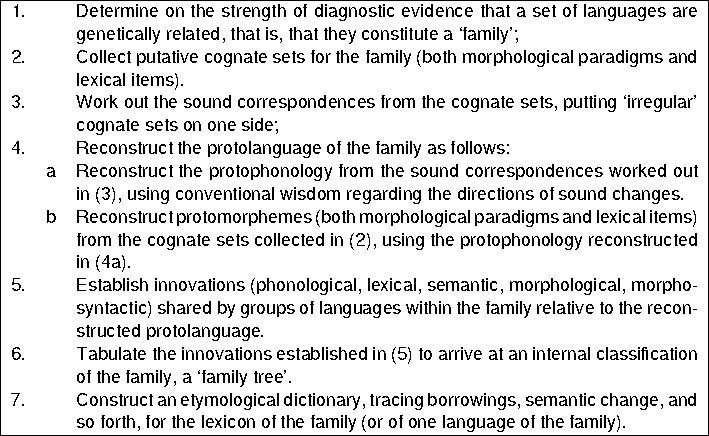
\includegraphics[width=\textwidth]{img/rodu.pdf}



\vspace{0.5cm}\par\noindent\textbf{Visualisierung des Workflows von\vspace{0.5cm}
\href{http://bibliography.lingpy.org?key=Ross1996}{Ross und Durie
(1996)}}

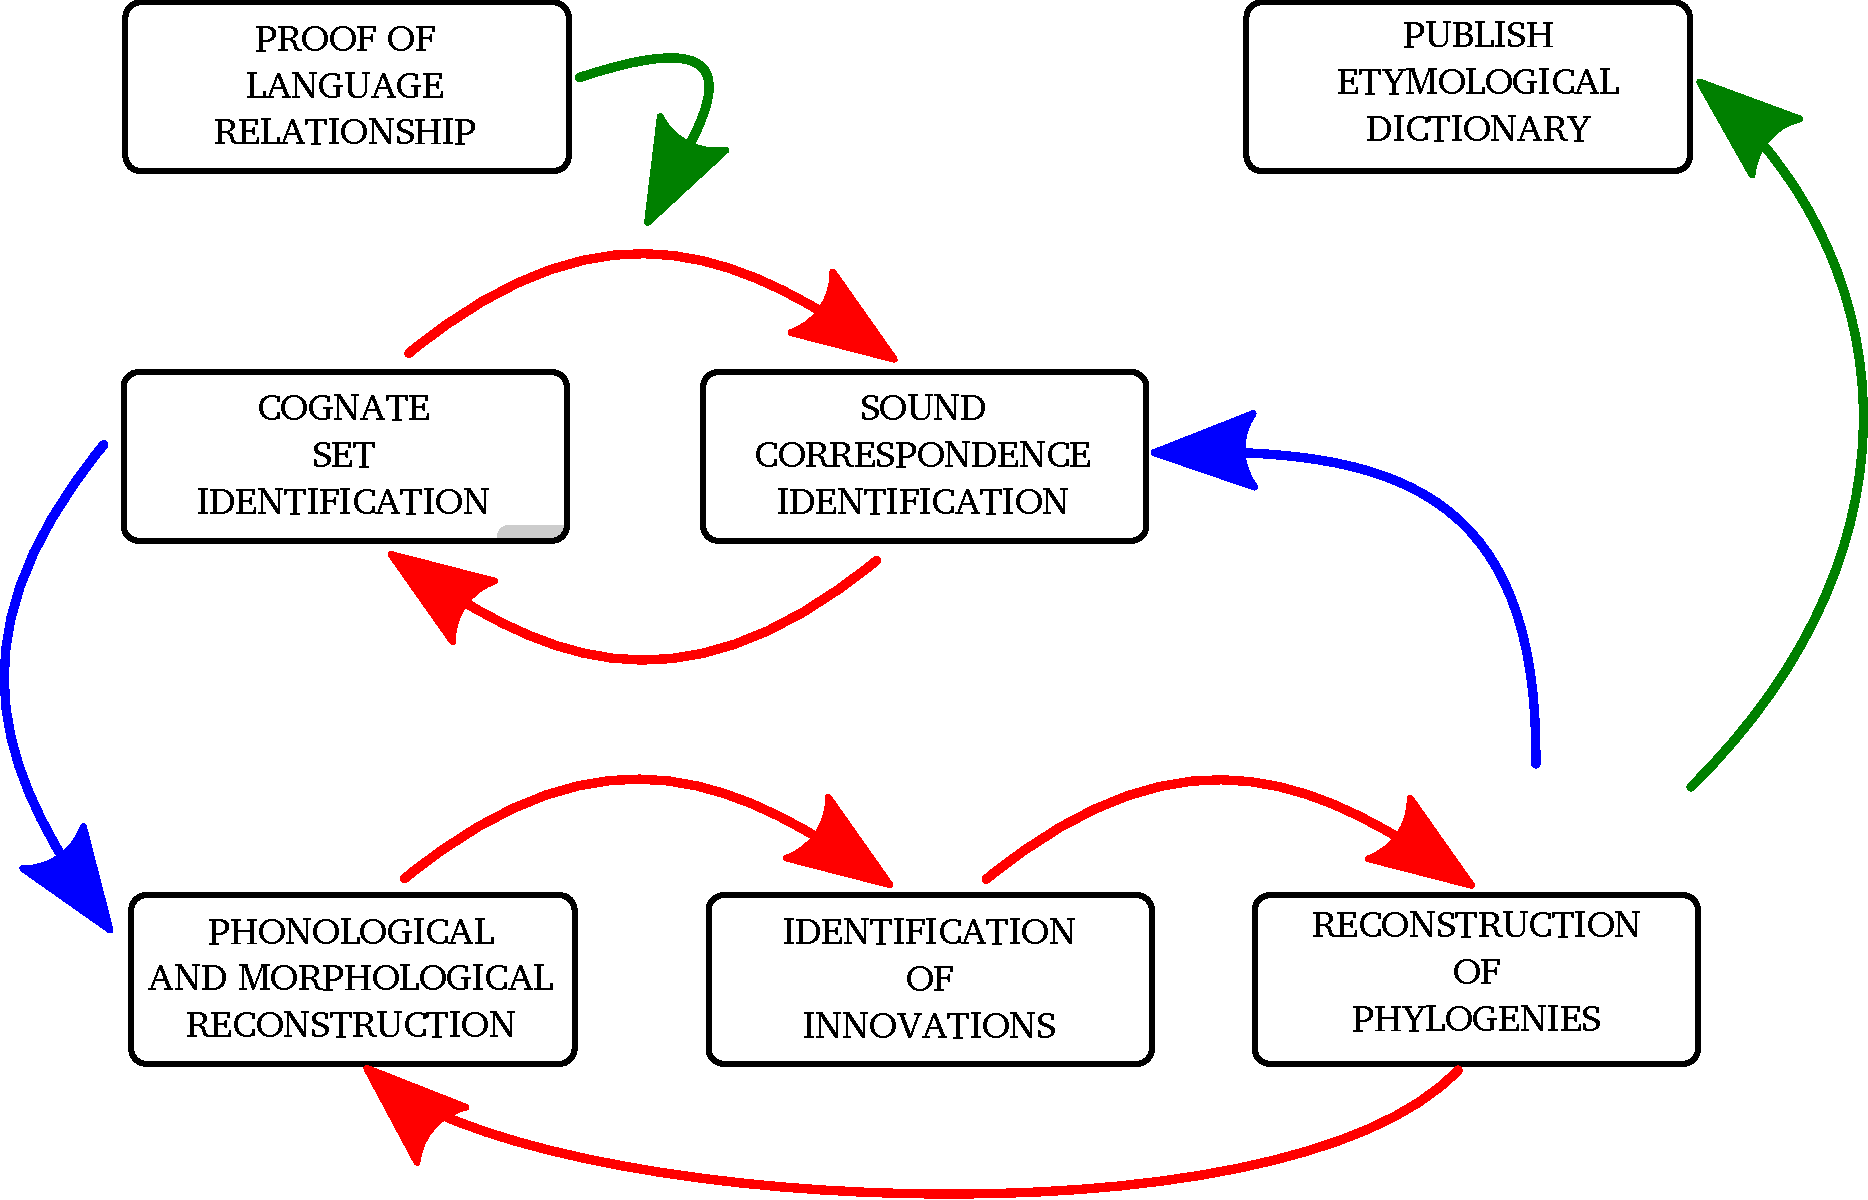
\includegraphics[width=\textwidth]{img/ross-durie-workflow.pdf}



\vspace{0.5cm}\par\noindent\textbf{Vereinfachter Workflow\vspace{0.5cm}
\href{http://bibliography.lingpy.org?key=List2014d}{(List 2014)}}

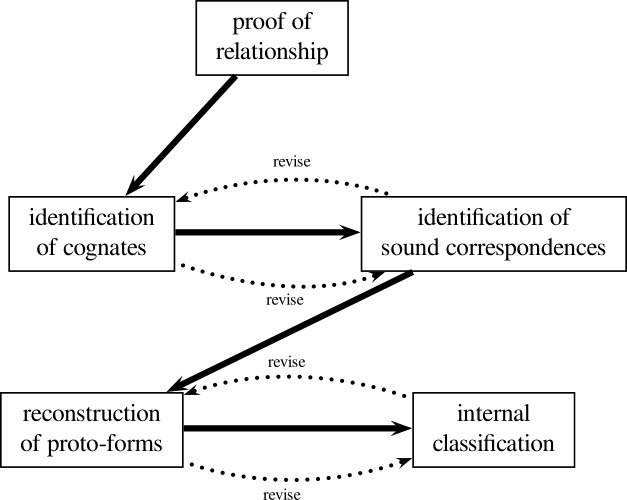
\includegraphics[width=\textwidth]{img/cm-simplified.png}

\subsection{\texorpdfstring{{Sequenzalinierung}}{Sequenzalinierung}}

\subsubsection{\texorpdfstring{{Sequenzen und
Sequenzvergleiche}}{Sequenzen und Sequenzvergleiche}}

\vspace{0.5cm}\par\noindent\textbf{Sequenzen: Definition (vgl.\vspace{0.5cm}
\href{http://bibliography.lingpy.org?key=Boeckenbauer2003}{Böckenbauer
und Bongartz 2003: 30f})}

\vspace{0.5cm}\par\noindent\textbf{Definition:} Ein \emph{Alphabet} ist eine nicht-leere endliche\vspace{0.5cm}
Menge deren Elemente \emph{Buchstaben} genannt werden. Eine
\emph{Sequenz} ist eine geordnete Liste von Buchstaben, die aus dem
Alphabet gezogen werden. Die Elemente von Sequenzen werden
\emph{Segmente} genannt, die \emph{Mächtigkeit} einer Sequenz ist die
Anzahl ihrer unterschiedlichen Buchstaben, und die \emph{Länge} einer
Sequenz ist die Anzahl ihrer Segmente.



\vspace{0.5cm}\par\noindent\textbf{Sequenzen als Perlenketten}\vspace{0.5cm}

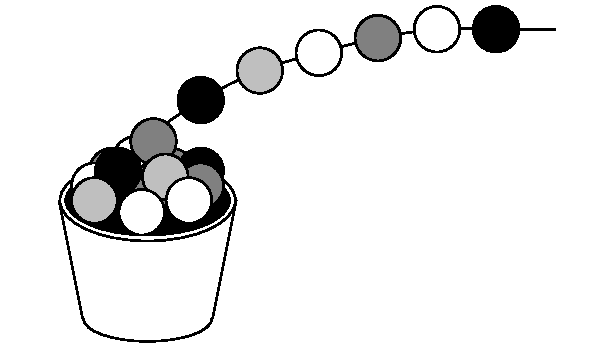
\includegraphics[width=\textwidth]{img/kette.pdf}


\vspace{0.5cm}\par\noindent\textbf{Vergleich von Sequenzen mit gleicher Länge}\vspace{0.5cm}

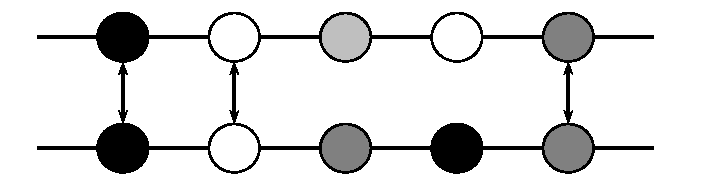
\includegraphics[width=\textwidth]{img/hamming.pdf}



\vspace{0.5cm}\par\noindent\textbf{Vergleich von Sequenzen mit unterschiedlicher Länge}\vspace{0.5cm}

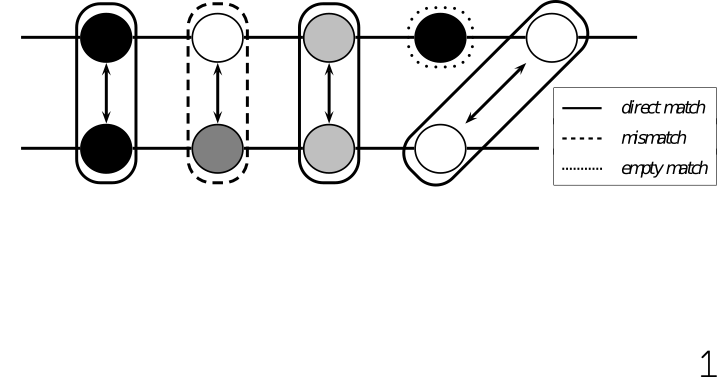
\includegraphics[width=\textwidth]{img/matchings.png}


\subsubsection{\texorpdfstring{{Alinierung}}{Alinierung}}

\vspace{0.5cm}\par\noindent\textbf{Definitionsversuch}\vspace{0.5cm}

\begin{quote}
Eine \emph{Alinierung} von $n$ ($n\textgreater{}1$) Sequenzen ist
eine $n$-reihige Matrix, in der alle Sequenzen dergestalt angeordnet
werden, dass alle matchenden Segmente in derselben Spalte erscheinen,
während nicht-matchende Segmente, die aus leeren Matches resultieren,
durch Gap-Symbole angezeigt werden. (vgl
\href{http://bibliography.lingpy.org?key=Gusfield1997}{Gusfield 1997:
216})
\end{quote}



\vspace{0.5cm}\par\noindent\textbf{Beispiel}\vspace{0.5cm}

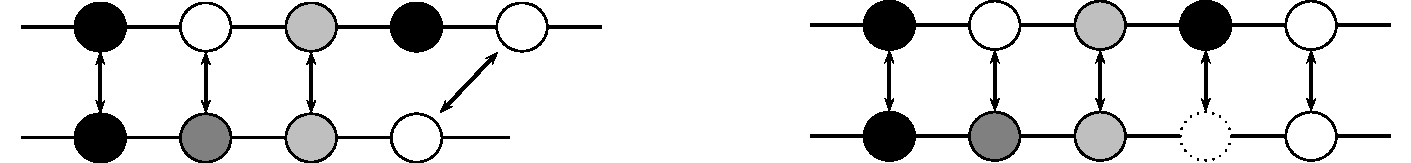
\includegraphics[width=\textwidth]{img/alignment.pdf}



\vspace{0.5cm}\par\noindent\textbf{Preisfrage}\vspace{0.5cm}

Die Levenshtein-Distanz zwischen zwei Sequenzen $S\_1$ und $S\_2$
ist definiert als die Anzahl von Editieroperationen, die notwendig ist,
um $S₁$ in $S\_2$ zu transformieren. Mit Hilfe des Konzepts der
Alinierung lässt sich dieses Distanzmaß leicht auf die Hamming-Distanz
zurückführen. Wie genau?


\subsubsection{\texorpdfstring{{Phonetische
Alinierung}}{Phonetische Alinierung}}

Obwohl Alinierungsanalysen eine der allgemeinsten Möglichkeiten
darstellen, Sequenzen zu vergleichen, steckt ihre Verwendung in der
historischen Linguistik noch in den Kinderschuhen. Natürlich alinieren
historische Linguisten eigentlich \emph{immer} Wörter und haben dies
auch schon immer getan, da ohne Alinierung überhaupt keine regulären
Lautkorrespondenzen ermittelt werden könnten. Der Sprachvergleich
basierte lange Zeit jedoch eher auf einer impliziten Alinierung, die
selten visualisiert wurde, und wenn doch, dann nur aus illustrativen
Zwecken.



\vspace{0.5cm}\par\noindent\textbf{Schwierigkeiten der phonetischen Alinierung}\vspace{0.5cm}

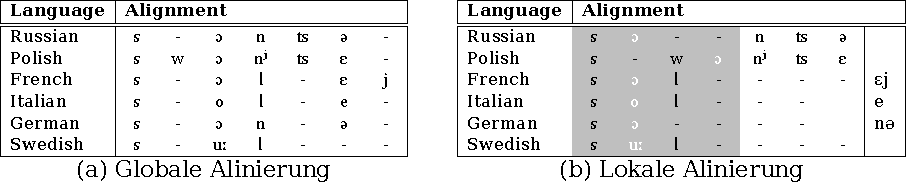
\includegraphics[width=\textwidth]{img/phonalign.pdf}



\vspace{0.5cm}\par\noindent\textbf{Substantielle und strukturelle Ähnlichkeit}\vspace{0.5cm}

\begin{itemize}
\itemsep1pt\parskip0pt\parsep0pt
\item
  die Wörter ``schlafen'' und ``Flaschen'' sind recht ähnlich
\item
  die Wörter ``Obst'' und ``Post'' auch
\item
  die Wörter ``Kerker'' und ``Tanten'' sind sich auch recht ähnlich,
  aber auf andere Art und Weise
\end{itemize}

\vspace{0.5cm}\par\noindent\textbf{Die beiden unterschiedlichen Formen von Ähnlichkeit können wir\vspace{0.5cm}
``substantielle'' vs. ``strukturelle'' Ähnlichkeit nennen.}



\vspace{0.5cm}\par\noindent\textbf{Heuristiken für strukturelle Ähnlichkeiten}\vspace{0.5cm}

Beim Alinieren in der historischen Linguistik ist es wichtig, der
Tatsache Rechnung zu tragen, dass substantielle Ähnlichkeit zwischen
Lauten nicht notwendigerweise auch auf deren Kognazität hinweist. Nur,
wenn zwei Segmente auch systematisch (also in den Sprachsystemen)
korrespondieren, sollten sie tatsächlich als ähnlich angesehen werden.
In den Schritten des Sprachvergleichs kann diese systematische
Ähnlichkeit jedoch schwer ermittelt werden, denn zu Beginn eines
Sprachvergleichs sind weder die kognaten Wörter bekannt, noch die
regulär korrespondierenden Laute.



\vspace{0.5cm}\par\noindent\textbf{Dolgopolskys Lautklassen}\vspace{0.5cm}

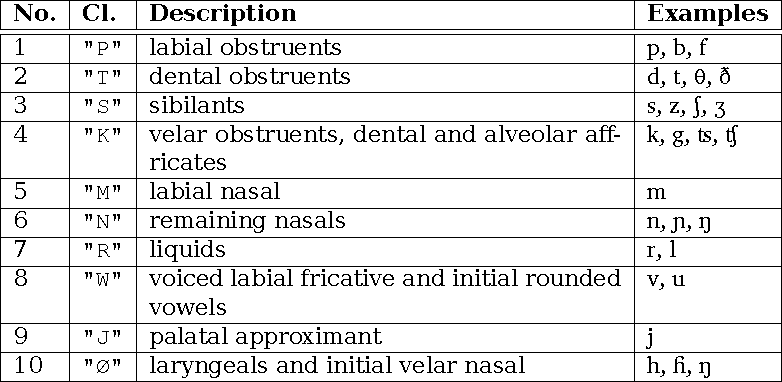
\includegraphics[width=\textwidth]{img/dolgopolsky.pdf}

